\documentclass[oneside]{amsart}
\usepackage[left=1.25in,right=1.25in,top=0.75in,bottom=0.75in]{geometry}
\linespread{1.05}
\usepackage{graphicx}
\usepackage{mathtools}
\usepackage{tcolorbox}
\usepackage{mathpazo}
\usepackage{euler}
\usepackage{amssymb,latexsym,amsmath,amsthm}
\usepackage{mathrsfs}
\usepackage{xcolor}
\usepackage{graphicx}
\usepackage{hyperref}
\hypersetup{
    colorlinks = true,
    linkbordercolor = {red}
}
\usepackage{xstring}
\usepackage{xparse}
\usepackage{mathrsfs}
% \definecolor{brightmaroon}{rgb}{0.76, 0.13, 0.28}
% \usepackage[linktocpage=true,colorlinks=true,hyperindex,citecolor=blue,linkcolor=brightmaroon]{hyperref}
%\usepackage{fullpage}
% \usepackage[a4paper, total={5.5in, 9in}]{geometry}
\usepackage{tikz-cd}
\theoremstyle{definition}
%% this allows for theorems which are not automatically numbered
\newtheorem{defi}{Definition}[section]
\newtheorem{theorem}{Theorem}[section]
\newtheorem{lemma}{Lemma}[section]
\newtheorem{obs}{Observation}
\newtheorem{exercise}{Exercise}[section]
\newtheorem{rem}{Remark}[section]
\newtheorem{construction}{Construction}[section]
\newtheorem{prop}{Proposition}[section]
\newtheorem{coro}{Corollary}[section]
\newtheorem{disc}{Discussion}[section]
\DeclareMathOperator{\spec}{Spec}
\DeclareMathOperator{\im}{im}
\DeclareMathOperator{\obj}{obj}
\DeclareMathOperator{\ext}{Ext}
\DeclareMathOperator{\Lim}{Lim}
\DeclareMathOperator{\Int}{Int}
\DeclareMathOperator{\tor}{Tor}
\DeclareMathOperator{\ann}{ann}
\DeclareMathOperator{\id}{id}
\DeclareMathOperator{\proj}{Proj}
\DeclareMathOperator{\gal}{Gal}
\DeclareMathOperator{\coker}{coker}
\newcommand{\degg}{\textup{deg}}
\newtheorem{ex}{Example}[section]
%% The above lines are for formatting.  In general, you will not want to change these.
%%Commands to make life easier
\newcommand{\RR}{\mathbf R}
\newcommand{\aff}{\mathbf A}
\newcommand{\ff}{\mathbf F}
\usepackage{mathtools}
% \newcommand{\ZZ}{\mathbf Z}
\newcommand{\pring}{k[x_1, \ldots , x_n]}
\newcommand{\polyring}{[x_1, \ldots , x_n]}
\newcommand{\poly}{\sum_{\alpha} a_{\alpha} x^{\alpha}} 
\newcommand{\ZZn}[1]{\ZZ/{#1}\ZZ}
% \newcommand{\QQ}{\mathbf Q}
\newcommand{\rr}{\mathbb R}
\newcommand{\cc}{\mathbb C}
\newcommand{\complex}{\mathbf {C}_\bullet}
\newcommand{\nn}{\mathbb N}
\newcommand{\zz}{\mathbb Z}
\newcommand{\PP}{\mathbb  P}
\newcommand{\cat}{\mathbf{C}}
\newcommand{\ca}{\mathbf}
\newcommand{\zzn}[1]{\zz/{#1}\zz}
\newcommand{\qq}{\mathbb Q}
\newcommand{\calM}{\mathcal M}
\newcommand{\latex}{\LaTeX}
\newcommand{\V}{\mathbf V}
\newcommand{\tex}{\TeX}
\newcommand{\sm}{\setminus} 
\newcommand{\dom}{\text{Dom}}
\newcommand{\lcm}{\text{lcm}}
\DeclareMathOperator{\GL}{GL}
\DeclareMathOperator{\cl}{cl}
\DeclareMathOperator{\Hom}{Hom}
\DeclareMathOperator{\aut}{Aut}
\DeclareMathOperator{\SL}{SL}
\DeclareMathOperator{\inn}{Inn}
\DeclareMathOperator{\card}{card}
\newcommand{\sym}{\text{Sym}}
\newcommand{\ord}{\text{ord}}
\newcommand{\ran}{\text{Ran}}
\newcommand{\pp}{\prime}
\newcommand{\lra}{\longrightarrow} 
\newcommand{\lmt}{\longmapsto} 
\newcommand{\xlra}{\xlongrightarrow} 
\newcommand{\gap}{\; \; \;}
\newcommand{\Mod}[1]{\ (\mathrm{mod}\ #1)}
\newcommand{\p}{\mathfrak{p}} 
\newcommand{\rmod}{\textit{R}-\textbf{Mod}}
\newcommand{\idealP}{\mathfrak{P}}
\newcommand{\ideala}{\mathfrak{a}}
\newcommand{\idealb}{\mathfrak{b}}
\newcommand{\idealA}{\mathfrak{A}}
\newcommand{\idealB}{\mathfrak{B}}
\newcommand{\X}{\mathfrak{X}}
\newcommand{\idealF}{\mathfrak{F}}
\newcommand{\idealm}{\mathfrak{m}}
\newcommand{\s}{\mathcal{S}}
\newcommand{\cha}{\text{char}}
\newcommand{\ccc}{\mathfrak{C}}
\newcommand{\idealM}{\mathfrak{M}}
\tcbuselibrary{listings,theorems}
\usetikzlibrary{decorations.pathmorphing} 
\newcommand{\overbar}[1]{\mkern 1.5mu\overline{\mkern-1.5mu#1\mkern-1.5mu}\mkern 1.5mu}

%Itemize gap:

% \pagecolor{black}
% \color{white}
% Author info

\title{Math 425A HW9, Oct. 28, 6PM}
\author{Juan Serratos}
\date{October 15, 2022 \\ {Department of Mathematics, University of Southern California}}
\address{Department of Mathematics, University of Southern California, 
Los Angeles, CA 90007}
\begin{document}
\maketitle
\setcounter{tocdepth}{4}
\setcounter{secnumdepth}{4}
 \section{Chapter 4}

\begin{tcolorbox}[colback=black!5!white,colframe=black!75!black,title= Chapter $4$; $\S 6.1$: Exercise $6.1.$] Let $\mathcal A$ be a collection of convex subsets of a real vector space $V$ . Show that $B:= \bigcap_{A \in \mathcal A} A$ is convex.
\tcblower 
\begin{proof}
	Clearly, $ \bigcap_{A \in \mathcal A} A$ is still a subset of $V$ as for all $A \in \mathcal A$ we have $A$ is a subset of $V$. Now let $a, b \in \bigcap_{A \in \mathcal A} A$ and $t \in \rr$ such that $0 < t < 1$. Then we have that $(1-t)a + tb \in A$ for all $A \in \mathcal A$ by construction of $\mathcal A$. Thus we have that $(1-t)a+tb \in \bigcap_{A \in \mathcal A} A$. 
\end{proof}
\end{tcolorbox}

\begin{tcolorbox}[colback=black!5!white,colframe=black!75!black,title= Chapter $4$; $\S 6.2$: Exercise $6.2.$]  Let $(X, d)$ be a metric space and let $A$ and $B$ be disjoint subsets of $X$. Prove that if $A$ and $B$ are both open in $X$, then $A$ and $B$ are separated.
\tcblower 
\begin{proof} Suppose that $A$ and $B$ are both open in $X$. WLOG, suppose that $\cl_X(A) \cap B \neq \varnothing$. Then we have some $\ell \in \cl_X(A) \cap B$; thus we have $\ell \in B$ and for any open neighborhood of $\ell \in U$ then $U \cap A \neq \varnothing$. But as $B$ is itself an open neighborhood of $\ell$ as $\ell$ is in the intersection, then $B \cap A \neq \varnothing$; this contradicts our assumption that $A$ and $B$ are disjoint. Therefore we have that $\cl_X(A) \cap B = \varnothing$. To show that $\cl_X(B) \cap A = \varnothing$ follows nearly the exact same argument. Hence we have that $\cl_X(A) \cap B = \varnothing$ and $\cl_X(B) \cap A = \varnothing$, i.e. $A$ and $B$ are separated. 
\end{proof}
\end{tcolorbox}
 
 
 \begin{tcolorbox}[colback=black!5!white,colframe=black!75!black,title= Chapter $4$; $\S 6.2$: Exercise $6.3.$]  Let $E$ be a connected subset of a metric space $(X, d)$. Show that $\overbar{E}$ is connected.
\tcblower 
\begin{proof} Suppose we can write $\overbar{E} = A \cup B$ where $A \cap \overbar{B} = \varnothing = \overbar {A} \cap B$. We can write $E  = (A \cap E ) \cup (B \cap E)$, and we still have that $(A \cap E)$ and $(B \cap E)$ are separated. Thus as $E$ is connected, either $A \cap E = \varnothing$ or $B \cap E = \varnothing$. WLOG, suppose $A \cap E = \varnothing$. Then $E = B \cap E$, which implies that $E \subseteq B$ and so $\overline{E} \subseteq \overline{B}$. So as $A \cap \overline{B} = \varnothing$, then $A \cap \overline{E} = \varnothing$. Thus if we let $\ell \in \overline{E}$, then $\ell \in B$ (as if $\ell \in A$ then we have a contradiction), and hence $\overline{E} = B$, which means that $\overline{E}$ is connected. 
\end{proof}
\end{tcolorbox}
 \begin{tcolorbox}[colback=black!5!white,colframe=black!75!black,title= Chapter $4$; $\S 6.2$: Exercise $6.4.$]   Let $(X,d)$ be a metric space, and let $\mathcal C$ be a collection of connected subsets of $X$. Assume $A = \bigcap _{C\in \mathcal C} C $ is nonempty. Show that $B =\bigcup _{C\in \mathcal C} C $ is connected.
\tcblower 
\begin{proof} By contradiction, suppose that $B$ is not connected. That is, suppose we can write $B = E \cup F$ where $ \overline{E} \cap F = \overline{F} \cap E = \varnothing$. Then for all $C_k$ in $\mathcal C$, we have $C_k \subseteq E \cup F$. By Theorem 6.4, we have that $C_k \subseteq E$ or $C_k \subseteq F$. WLOG, let $C_k \subseteq E$. Then $C_k = (C_k \cap E) \cup (C_k \cap F)$, meaning that $C_k \cap F = \varnothing$ and $C_k = C_k \cap E$. As we assumed $B = E \cup F$ with both nonempty, then we have $C_k \subseteq E$ and $C_l \subseteq F$ where $k \neq l$. But this additionally means that $C_k \cap C_l  = \varnothing$ by Theorem 6.4, which is a contradiction. Thus $B$ is connected. 
\end{proof}
\end{tcolorbox}

\begin{tcolorbox}[colback=black!5!white,colframe=black!75!black,title= Chapter 4; $\S 6.2$: Exercise $6.5.$]   Let $X = \rr^2$. Give an example of a connected subset $E$ of $X$, such that $\Int_ X (E)$ is not connected. Prove both that your set $E$ is connected and that its interior is not. (Hint: Consider the union of two convex sets joined at a point. You may assume without proof the fact that convexity implies connectedness in $\rr^2$.)
\tcblower 
\begin{proof}  Consider $\mathcal M_1 = \{ (x,y) \in \rr^2 \colon x \geq 0, y \geq 0 \} $ and $\mathcal M_2 = \{ (x,y) \in \rr^2 \colon x \leq 0, y \leq 0 \}$. We glue these two $\mathcal M = \mathcal M_1 \cup \mathcal M_2 \subseteq \rr^2 $. Firstly, let $(a,b), (x,y) \in \mathcal M_1$ where $\ell_1 = (a,b)$ and $\ell_2 = (x,y)$, and let $t \in \rr$ such that $0 < t <1$. Then $(1-t)\ell_1 + t \ell_2$ will clearly be always be bigger than or equal to $0$ as $t-1 > 0$ and $\ell_1, \ell_2 \geq 0$. So $\mathcal M_1$ is convex.  For $\mathcal M_2$, let $\alpha_1 = (a,b)$ and $\alpha_2 = (x,y)$ be in $\mathcal M _2$ with $t \in \rr$ such that $0 < t < 1$. Then $(1-t) \alpha_1 + t\alpha_2$ is always less than or equal to zero clearly. So, by Exercise 6.4, $\mathcal M = \mathcal M_1 \cup \mathcal M_2$ is connected since convexity implies connected in $\rr^2$. We claim that $\Int_{\rr^2} (\mathcal M) = \Int_{\rr^2} (\mathcal M_1) \cup \Int_{\rr^2}(\mathcal M_2)$. Let $x \in \mathcal \Int_{\rr^2} (\mathcal M)$. Then $x \in \mathcal M$ and there exists an open ball $B_{\rr^2}(x, \epsilon) \subseteq \mathcal M = \mathcal M_1 \cup \mathcal M_2$. We know that, as $\mathcal M_1$ and $\mathcal M_2$ are tangent to one another, if $B_{\rr^2}(x, \epsilon) \subseteq \mathcal M_1 \cap \mathcal M_2 = \{ (0,0) \}$, then $B_{\rr^2}(x, \epsilon) = \{ (0,0) \}$. So $B_{\rr^2}(x,\epsilon) \subseteq \mathcal M_1$ (and also $B_{\rr^2} (x,\epsilon) \subseteq \mathcal M_2)$. Thus we have the forward inclusion since (if we had the only other case, the trivial case) $ B_{\rr^2} (x, \epsilon) \subseteq \mathcal M_1 \cup \mathcal M_2$ where $B_{\rr^2} (x, \epsilon) \subseteq \mathcal M_1$ (or $B_{\rr^2}(x, \epsilon) \subseteq \mathcal M_2$), then $x \in \Int_{\rr^2}(\mathcal M_1)$. Now for the backwards direction, let $\ell \in \Int_{\rr^2}(\mathcal M_1) \cup \Int_{\rr^2}(\mathcal M_2)$. WLOG, let $\ell \in \Int_{\rr^2} (\mathcal M_1)$. Then we have $ \ell \in \mathcal M_1 $ such that there is an open $\epsilon$-neighborhood $B_{\rr^2}(\ell, \epsilon) \subseteq \mathcal M_1$, but as $\mathcal M_1 \subseteq \mathcal M_1 \cup \mathcal M_2 = \mathcal M$, then we have that $\ell \in \mathcal M$ and $B_{\rr^2} (\ell, \epsilon) \subseteq \mathcal M$. Thus $\ell \in  \Int_{\rr^2} ( \mathcal M)$. Therefore we have the equality of sets. Lastly, $\overline{\Int_{\rr^2} (\mathcal M _1)} \cap \Int_{\rr^2} ( \mathcal M_2 ) = \mathcal M_1 \cap \Int_{\rr^2} ( \mathcal M_2) = \varnothing$, and similarly, $\overline{\Int_{\rr^2} (\mathcal M _2)} \cap \Int_{\rr^2} ( \mathcal M_1 ) = \mathcal M_2 \cap \Int_{\rr^2} ( \mathcal M_1) = \varnothing$. Thus we have written $\Int_{\rr^2} (\mathcal M)$ as the union of two disjoint, nonempty, separated sets, and so $\Int_{\rr^2} (\mathcal M)$ is not connected. 
\end{proof}
\end{tcolorbox}
\begin{figure}[h!] 
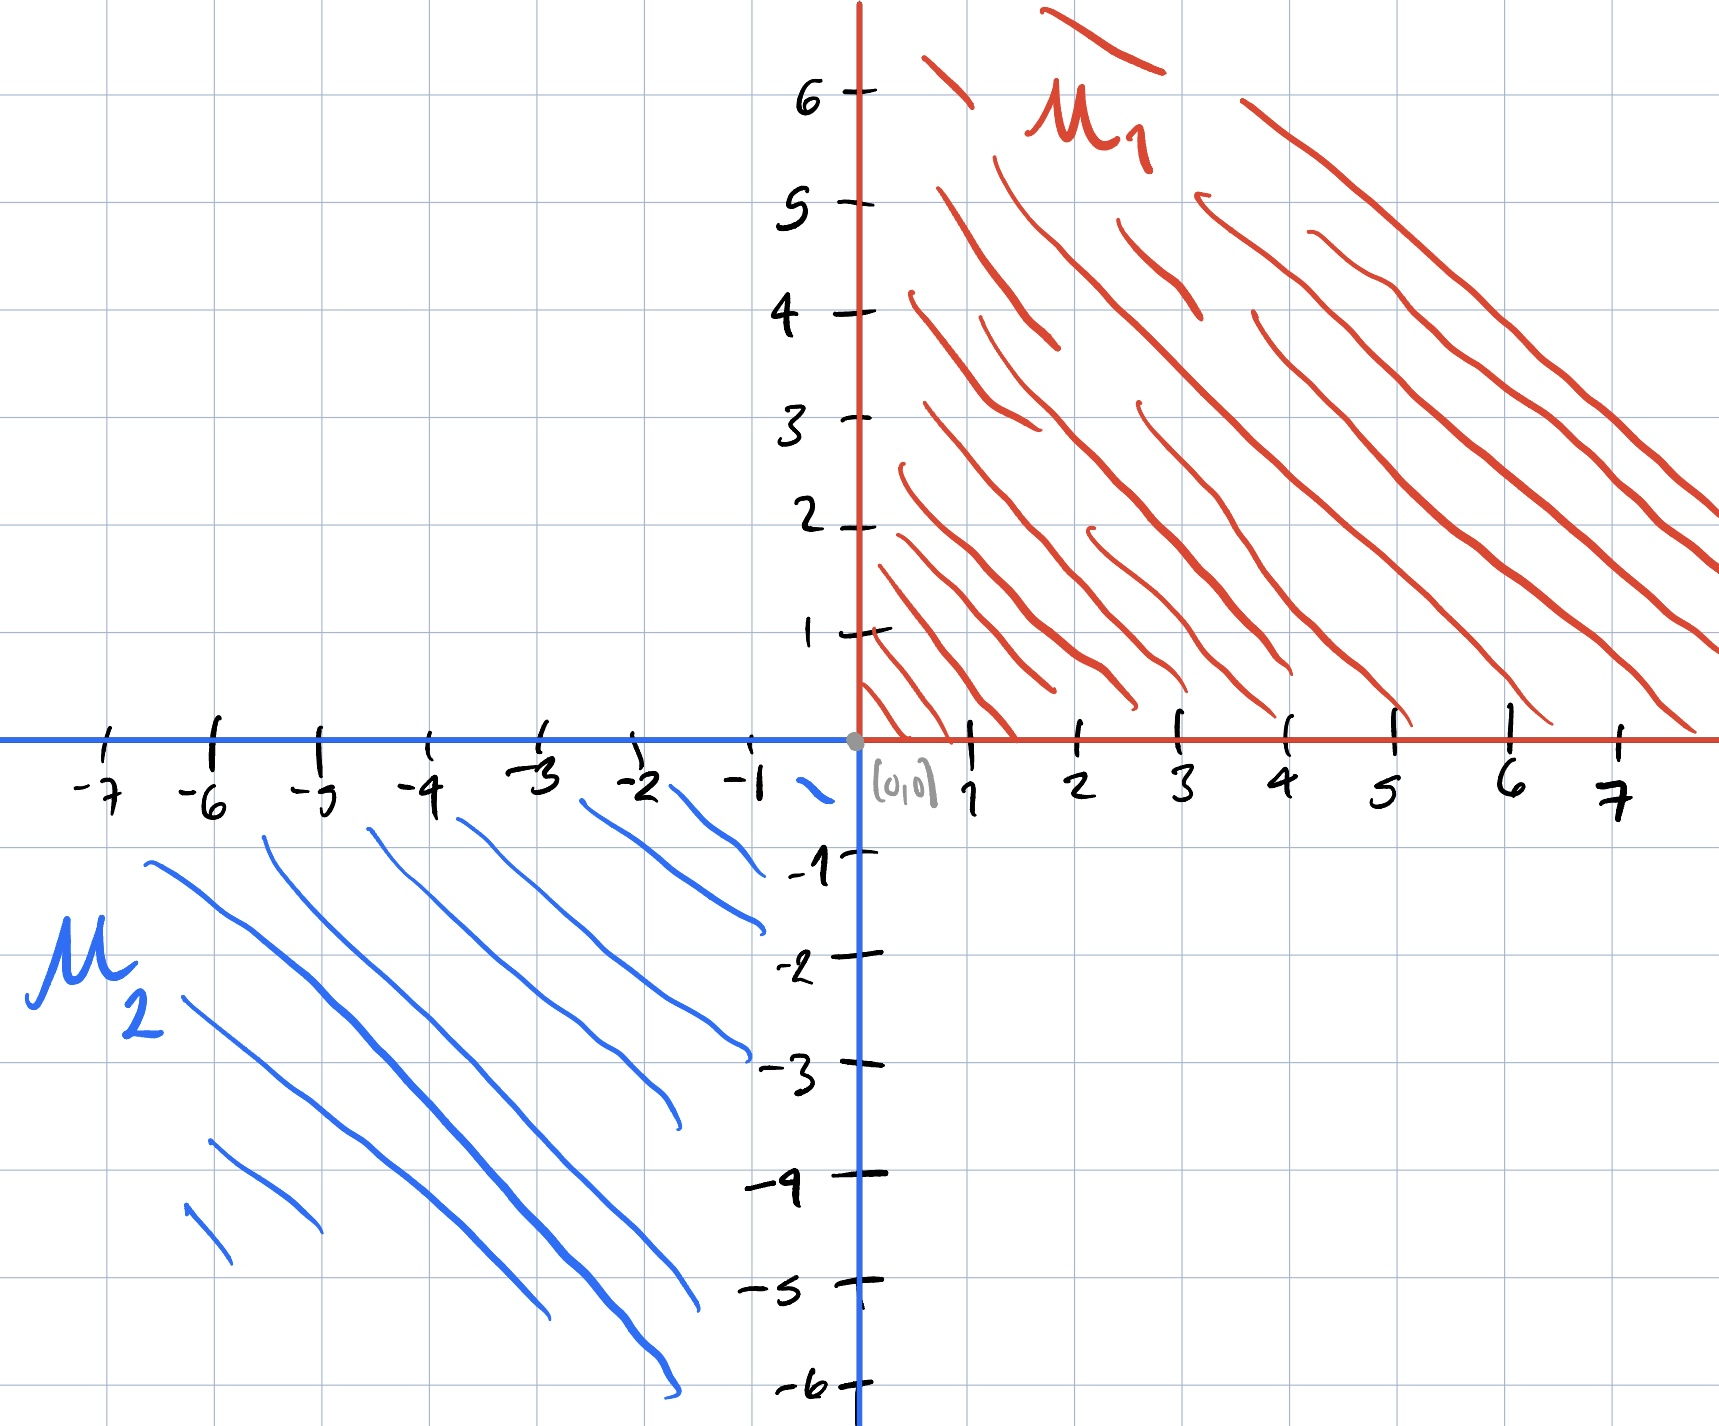
\includegraphics[scale = .12]{IMG_0710.jpg} 
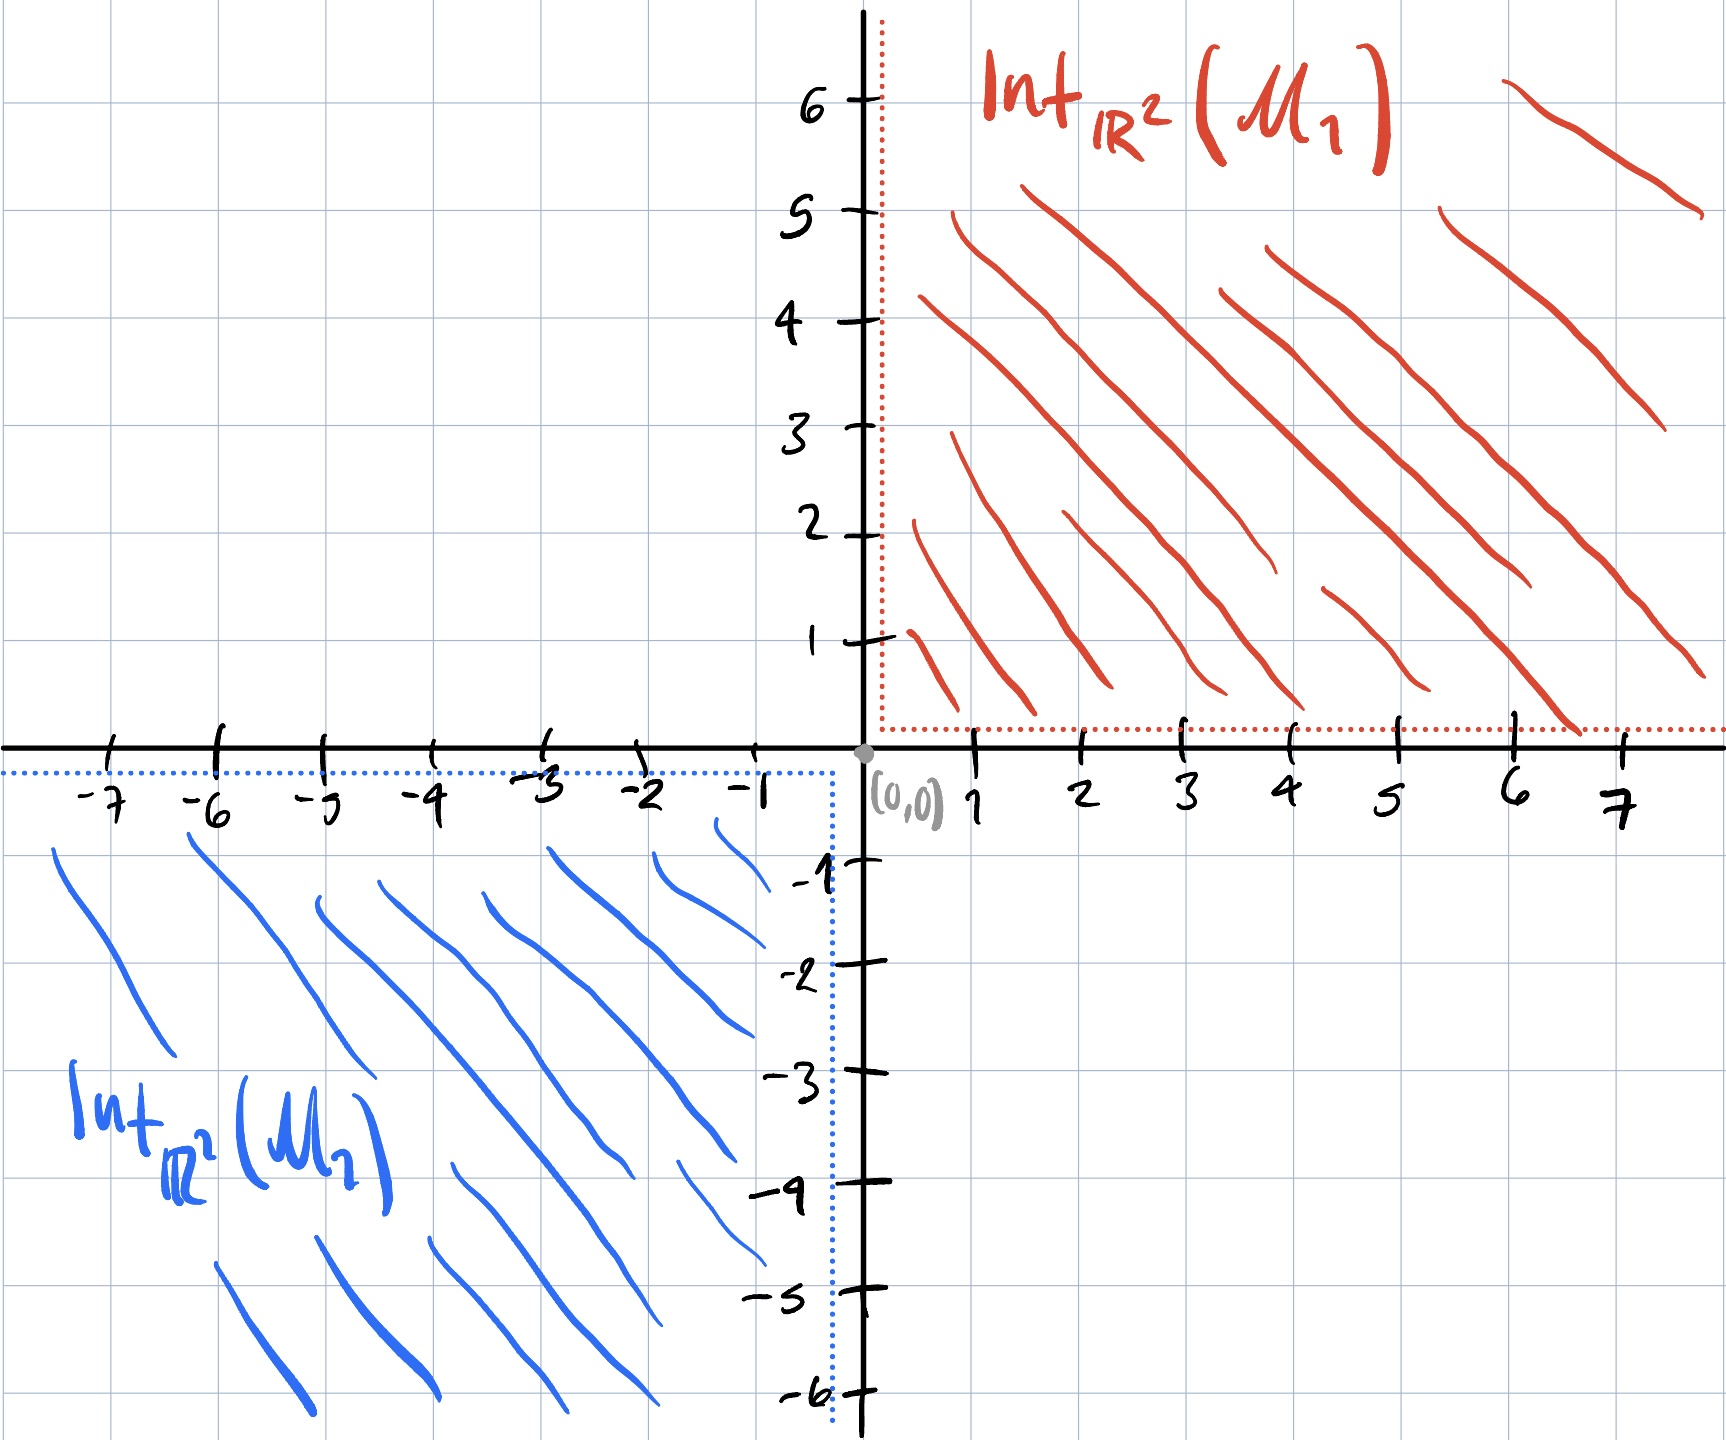
\includegraphics[scale = .12]{IMG_0711.jpg}
\caption{The image to the left depicts $\mathcal M_1$ and $\mathcal M_2$ for Exercise 6.5, and image to the left depicts the interiors of the sets.}
\end{figure}
 \section{Chapter 5}
 
  \begin{tcolorbox}[colback=black!5!white,colframe=black!75!black,title= Chapter 5; $\S 1.1$: Exercise $1.1.$]  Let $(X, d_X)$ and $(Y, d_Y)$ be metric spaces, and let $E$ be a subset of $X$. Let $f \colon  E \to  Y$ be a function, and let $p$ be a limit point of $E$ in $X$. Prove that $f(x) \to q$ as $x \to p$ if and only if for every $\epsilon > 0$, there exists $\delta > 0$ such that $x \in E$ and $0 < d_X(x,p) < \delta$ imply together that $d_Y (f(x),q) < \epsilon$.
\tcblower 
\begin{proof} $(\Rightarrow )$ Suppose that $\lim_{x \to p} f(x) = q$. Consider the open neighborhood $V = B_Y(q, \epsilon)$, where $\epsilon > 0$. Then we have some open neighborhood $p \in B_X(p, \delta) = U$ of $X$. So take $x \in B_X(p, \delta) \cap E \setminus \{ p \}$. Then $x \in E$ and $x \neq p$ with $d_X(x,p) < \delta$ (and as $x \neq p$, then we have $0 < d_X(x,p) < \delta )$. Moreover we have that $f(x) \in V = B_Y(q, \epsilon)$, and so $d_Y(f(x), q) < \epsilon$. Thus the forward direction is established. $(\Leftarrow)$ Suppose that for any $\epsilon > 0$ we have some $\delta > 0$ such that $x \in E$ and $0 < d_X(x,p) < \delta$ implies that $d_Y (f(x), q) < \epsilon$. Note that as $0 < d_X(x,p)$ for all such $x \in E$ then $x \neq p$. WLOG, consider the open neighborhood $B_Y(q, \epsilon)$ with $\epsilon > 0$ as assumed. Then by hypothesis we have an induced open neighborhood $B_X(p, \delta)$ where $0 < d_X(x,p) < \delta$ for all $x \in E$. As $x \neq p$, and $p \in \Lim_X(E)$, then $B_X(p, \delta) \cap E \setminus \{ p \} \neq \varnothing$. Lastly, by assumption, we have that $d_Y(f(x), q) < \epsilon$, which means that $f(x) \in B_Y(q, \epsilon)$. Hence the backwards assumption is established and we are done.
\end{proof}
\end{tcolorbox}



  \begin{tcolorbox}[colback=black!5!white,colframe=black!75!black,title= Chapter 5; $\S 2.1$: Exercise $2.1.$]  Let $(X, d_X)$ and $(Y, d_Y)$ be metric spaces; let $f \colon X \to Y$ be a function. Prove that $f$ is continuous at $p \in X$ if and only if $\epsilon > 0$, there exists $\delta > 0$ such that $x \in B_X(p, \delta)$ implies $f(x) \in B_Y(f(p), \epsilon)$.
\tcblower 
\begin{proof} $(\Rightarrow)$ Suppose that $f$ is continuous at $p \in X$. Then for the neighborhood $B_Y(f(p), \epsilon)$, where $\epsilon > 0$, we have that there exists a neighborhood $B_X(p, \delta)$ such that $x \in B_X(p, \delta)$, i.e. $x \in X$ such that $d_X(p,x) < \delta$, gives us that $f(x) \in B_Y(f(p), \epsilon)$. Thus the forward direction follows. $(\Leftarrow)$ Let $\epsilon > 0$. Consider the neighborhood $f(p) \in V = B_Y(f(p), \epsilon) \subseteq Y$. Then we have some $\delta > 0$ such that for $x$ being in the neighborhood $U = B_X(p, \delta)$, we have $f(x) \in V$. Thus, by definition, we have that $f$ is continuous at the point $p \in X$.
\end{proof}
\end{tcolorbox}

 \begin{tcolorbox}[colback=black!5!white,colframe=black!75!black,title= Chapter 5; $\S 2.1$: Exercise $2.2.$]  Assume $f \colon \rr \to \rr$ is a function satisfying $\lim_{h \to 0} [f(x+h) -f(x-h)] = 0$, for all $x \in \rr$. Does it follow that $f$ must be continuous? If so, give a proof; if not, give a counterexample.
\tcblower 
\begin{proof} We construct a function that satisfies this property: consider the function $\varphi  \colon \rr \to \rr $, where   
\[
\varphi (x) = \begin{cases}
	0 & \text{ if $x > 0$ or $x< 0$}\\
	1 & \text{ if $x =0$}x
\end{cases}
\]
Firstly, we can check that $\varphi$ satisfies a simple property: We claim that $\varphi (x) = \varphi (-x)$ for $x \in \rr$. WLOG, if $x > 0$, then $\varphi (x) = 0$, but multiplying the inequality by $-1$ gives us $-x< 0$ so $\varphi (-x) = 0$; thus $\varphi (x) = \varphi (-x)$ for $x \in \rr \setminus \{ 0 \}$. If $x = 0 \in \rr$, then $\varphi (x) = \varphi (0) = \varphi (-0) = \varphi (-x) = 0$. Now fix $x = 0$, then $\lim_{h \to 0} (\varphi(x+h) -\varphi(x-h) )= \lim _{h \to 0}  (\varphi(h) - \varphi(-h) )= \lim _{h \to 0}  (\varphi(h) - \varphi(h) ) = \lim_{h \to 0} (0 -0) = 0$. However, if we suppose that $\varphi$ is continuous at $x = 0$, then $\lim_{h \to 0} \varphi(h) = \varphi (0)$, but $\lim_{h \to 0} \varphi (h) = 0$ and $\varphi (0) = 1$, which is contradictory. Thus $\varphi $ cannot be continuous. 
\end{proof}
\end{tcolorbox}


 \begin{tcolorbox}[colback=black!5!white,colframe=black!75!black,title= Chapter 5; $\S 2.1$: Exercise $2.3.$]  Let $(X, d_X)$ and $(Y,d_Y)$ be metric spaces and $f \colon X \to Y$ a function.
 \begin{itemize}
 	\item [(a)] Show that $f$ is contiunous if and only if $f^{-1}(C)$ is closed in $X$ whenever $C$ is closed in $Y$.
 	\item [(b)] Show that $f \colon X \to Y$ is continuous if and only if $f (\overbar{A}) \subseteq \overbar{f(A)}$ for every subset $A$ of $X$.
 	\item [(c)] Consider the (continuous) function $g \colon \rr \to \rr$ given by $g(x) = \frac{1}{1+x^2}$. Give an example of a subset $A$ of $\rr$ such that $g(\overbar{A}) \neq \overbar{g(A)}$,
 \end{itemize}
\tcblower 
\begin{proof} (a) $(\Rightarrow)$ Suppose $f$ is continuous, and let $C$ be a closed subset in $Y$. Then we have that $Y \setminus C$ is open in $Y$, so $f^{-1} ( Y \setminus C)$ is open in $X$. Now, by Exercise 3.3.in Chapter 1 $\S 3.2$ we have that $f^{-1}(Y \setminus C) = f^{-1}(Y) \setminus f^{-1}(C)$, which is thus open in $X$. Moreover, clearly, we have that $f^{-1}(Y) = \{ x \in X \colon f(x) \in Y \} = X$, and so $f^{-1}(Y\setminus C) = X \setminus f^{-1}(C)$ is open in $X$. And $f^{-1}(C)$ is closed in $X$ if and only if $X \setminus f^{-1}(C)$ is open in $X$. Thus we're done. 

$(\Leftarrow)$ Suppose that whenever $C$ is closed in $Y$, then $f^{-1}(C)$ is closed in $X$. But $U$ is an open set of $Y$ if and only if $Y \setminus U$ is closed in $Y$. Furthermore, $f^{-1}(U)$ is open in $X$ if and only if $X \setminus f^{-1}(U)$ is closed in $X$. Clearly we have the statement the proposition as $Y \setminus U$ is closed in $Y$ and $X \setminus f^{-1}(U)$ is closed in $X$ by assumption.

(b) $(\Rightarrow)$ Suppose $f$ is continuous, and let $A \subseteq X$. Let $f(a) \in f(\overline{A})$. Then we have that $f(a) \in f(A)$, and so as $f$ is continuous then for any, wlog, open neighborhood $V$ of $f(a)$ we have some open neighborhood of $a \in U$ such that $x \in U $ implies $f(x) \in V$. As $a \in \overline{A}$, then for any open neighborhood $a \in U$, we have $U \cap A \neq \varnothing$; let $\ell$ be in this intersection. So $\ell \in U$ and $\ell \in A$, which means that $f(\ell) \in f(A)$ and $f(\ell) \in V$, i.e. $f(A) \cap V \neq \varnothing$. This proves that $f(a) \in \overline{f(A)}$. $(\Leftarrow)$ Suppose that for any subset $A \subseteq X$, we have $f(\overline{A}) \subseteq \overline{f(A)}$. Let $S$ be a closed set of $Y$. Then $ f^{-1}(S) \subseteq X$, and so by assumption we have $f(\overline{ f^{-1}(S)}) \subseteq \overline{ f(f(^{-1}(S) )} \subseteq \overline{S}$. Moreover, as $S$ is closed, then $S = \overline{S}$ and $f( \overline{f^{-1}(S) }) \subseteq S$. Now as a preimage preserves inclusions implies $\overline{f^{-1}(S)} \subseteq f^{-1}(S)$. So as $\overline{f^{-1}(S)} = f^{-1} (S) \cup (f^{-1}(S))^\prime$, we have $f^{-1}(S) = \overline{f^{-1}(S)}$. Thus $f^{-1}(S)$ is closed in $X$. Hence $f$ is continuous by part $(a)$ above.

(c) Consider the set $A = [1, \infty)$. Then $\overline{A} = [1, \infty ) = A$. So $g(\overline{A}) = \left( 0, \frac{1}{2} \right ] = g(A)$, while $ \overline{g(A)} = \overline{\left(0, \frac{1}{2} \right ]} = \left [0, \frac{1}{2} \right]$. Hence $g(\overbar{A}) \neq \overbar{g(A)}$. 
\end{proof}
\end{tcolorbox}






 \begin{tcolorbox}[colback=black!5!white,colframe=black!75!black,title= Chapter 5; $\S 2.1$: Exercise $2.4.$]  Let $(X, d_X)$ and $(Y, d_Y)$ be metric spaces, and let $f$ and $g$ be continuous functions from $X$ to $Y$. Assume $E$ is a dense subset of $X$.
\begin{itemize}
	\item [(a)] Prove that $f(E)$ is dense in $f(X)$. (Hint: Use Exercise 1.12 in Chapter 4 and Exercise 2.3 above.)
	\item [(b)] Prove that if $f(x) = g(x)$ for all $x \in E$, then $f(x) = g(x)$ for all $x \in X$.
\end{itemize}
\tcblower 
\begin{proof} (a) As $E \subseteq X$ then $f(E) \subseteq f(X) \subseteq Y$, and so $f(E)$ is dense in $f(X)$ if and only if $ f(X) \subseteq \overline{f(E)}$ (Exercise 1.12.). As $f$ is continuous then we have that $f(\overbar{E}) \subseteq \overbar{f(E)}$ (Exercise 2.3 (b)), but as $\overline{E}$ is dense in $X$, then $\overbar{E} = X$, so $f(X) \subseteq \overbar{f(E)}$. Therefore we have that $f(E)$ is dense in $f(X)$. 

(b) Let $\ell \in \overline{E}$. Then there is a sequence $\{l_n \}_{n=1}^\infty$ of $E$ such that $l_n \to \ell$ as $n \to \infty$. As $f$ is continuous, then $\lim_{n \to \infty} f(l_n) = f( \ell )$ and $\lim_{n\to \infty} g(l_n) = g (\ell )$. And as $l_n \in E$ for all $n \in \nn$, then we have $f(\ell) = g(\ell)$ by assumption. But as $E$ is dense in $X$, then we in fact have that for all $ q \in X = \overline{E}$ there is a sequence $(q_n)$ in $E$ where $q_n \to q$ and so $f(q) = g(q)$, as the work showed before.
\end{proof}
\end{tcolorbox}


\end{document}